\documentclass{beamer}
\usetheme{Madrid}

\usepackage{graphicx}
\graphicspath{{./images/}}
\usepackage{xcolor}
\usepackage{array}
\usepackage{amsfonts}
\usepackage{amssymb}
\usepackage{stmaryrd}
\usepackage[export]{adjustbox}
\usepackage{mathrsfs}
\usepackage{bbold}
\usepackage{tikz}
\usetikzlibrary{positioning,arrows.meta}

\tolerance=1
\emergencystretch=\maxdimen
\hyphenpenalty=10000
\hbadness=10000

\setbeamertemplate{caption}[numbered]

\title[ECD 415: Project Phase 1]{ECD 415: Project Phase 1} 
\subtitle{Zeroth Presentation -- July 2026}

\author[Group 01]{%
  \textbf{Presented by: Group 01}\\[6pt]
  AMAYA PRAMOD (KNR23EC013)\\
  HARIKESH O P (KNR23EC044)\\
  NANDANA JAYACHANDRAN (KNR23EC064)\\
  POOJA K L (KNR23EC111)%
}

\institute[GCE Kannur]{%
  \small Guided by: \textbf{Dr. Sajesh Kumar U}\\[6pt]
  \footnotesize Department of Electronics and Communication Engineering \\
  Government College of Engineering, Kannur%
}

\date[]{\color{blue}July 2026}

\begin{document}

%---------------- Title Slide ----------------
\begin{frame}
  \titlepage
\end{frame}

%---------------- Outline ----------------
\begin{frame}{Outline: Proposed Project Topics}
\begin{itemize}
  \item \textbf{Topic 1:} Edge AI Smart Battery Management System with Intelligent UPS
  \vspace{0.35cm}
  \item \textbf{Topic 2:} Embedded Electronics Diagnostic Instrument
  \vspace{0.35cm}
  \item \textbf{Topic 3:} Adaptive LoRa Mesh Emergency Communication Network
\end{itemize}
\vspace{0.5cm}
\begin{block}{\centering Presentation Structure per Topic}
  \centering \small Introduction $\;\bullet\;$ Problem Statement $\;\bullet\;$ Proposed Methodology $\;\bullet\;$ Block Diagram $\;\bullet\;$ Expected Outcomes $\;\bullet\;$ Applications
\end{block}
\end{frame}

%================ TOPIC 1 ================
\begin{frame}
  \begin{block}{\centering \huge Topic 1}
    \vspace{0.3cm}
    \centering \Large \textbf{Edge AI Smart Battery Management System with Intelligent UPS}
    \vspace{0.3cm}
  \end{block}
\end{frame}

\begin{frame}{Topic 1: Introduction}
\begin{itemize}
  \item \textbf{Widespread Applications:} Lithium-ion battery packs are extensively used in electric vehicles (EVs), renewable energy storage, robotics, and industrial backup systems.
  \vspace{0.25cm}
  \item \textbf{Limitations of Conventional BMS:} Provides only basic protection (over/under-voltage and over-current) with very limited insight into true battery health and long-term performance.
  \vspace{0.25cm}
  \item \textbf{Intelligent BMS Upgrade:} Integrates Edge AI, predictive analytics, and smart UPS capability directly on an advanced ESP32-S3 platform.
  \vspace{0.25cm}
  \item \textbf{Real-Time Intelligence:} Enables accurate SOC (State of Charge), SOH (State of Health), and RUL (Remaining Useful Life) estimation alongside pro-active on-device fault detection.
\end{itemize}
\end{frame}

\begin{frame}{Topic 1: Problem Statement}
\begin{itemize}
  \item \textbf{Basic Protection Only:} Conventional BMS acts mainly as a simple hardware cutoff device without diagnostic intelligence or forecasting abilities.
  \vspace{0.3cm}
  \item \textbf{Lack of Predictive Insights:} Unable to accurately evaluate cell degradation or predict Remaining Useful Life (RUL) under varying operating conditions.
  \vspace{0.3cm}
  \item \textbf{Financial \& Safety Risks:} Unprecedented cell aging leads to premature or delayed battery replacement, increasing overall lifecycle costs and sudden system failures.
  \vspace{0.3cm}
  \item \textbf{Proposed Need:} An Edge AI-based Intelligent BMS for sophisticated predictive analytics, real-time telemetry, and autonomous UPS switching management.
\end{itemize}
\end{frame}

\begin{frame}{Topic 1: Proposed Methodology}
\begin{itemize}
  \item \textbf{Data Acquisition:} Capture real-time cell voltage, current, and temperature using high-precision embedded sensors.
  \vspace{0.2cm}
  \item \textbf{Battery Monitoring:} Implement rigorous parameter estimation and multi-layer hardware safety protection algorithms.
  \vspace{0.2cm}
  \item \textbf{Edge AI Modeling:} Deploy lightweight machine learning models trained on historical cycling data for accurate SOH, RUL, and thermal fault prediction.
  \vspace{0.2cm}
  \item \textbf{On-Device Inference:} Perform ML inference directly on an ESP32-S3 processor for deterministic, low-latency execution without relying on cloud servers.
  \vspace{0.2cm}
  \item \textbf{Smart Management:} Facilitate intelligent UPS backup power switching, wireless telemetry data logging, and intuitive monitoring via a custom Flutter dashboard.
\end{itemize}
\end{frame}

\begin{frame}{Topic 1: Block Diagram}
\centering
\resizebox{0.95\linewidth}{!}{%
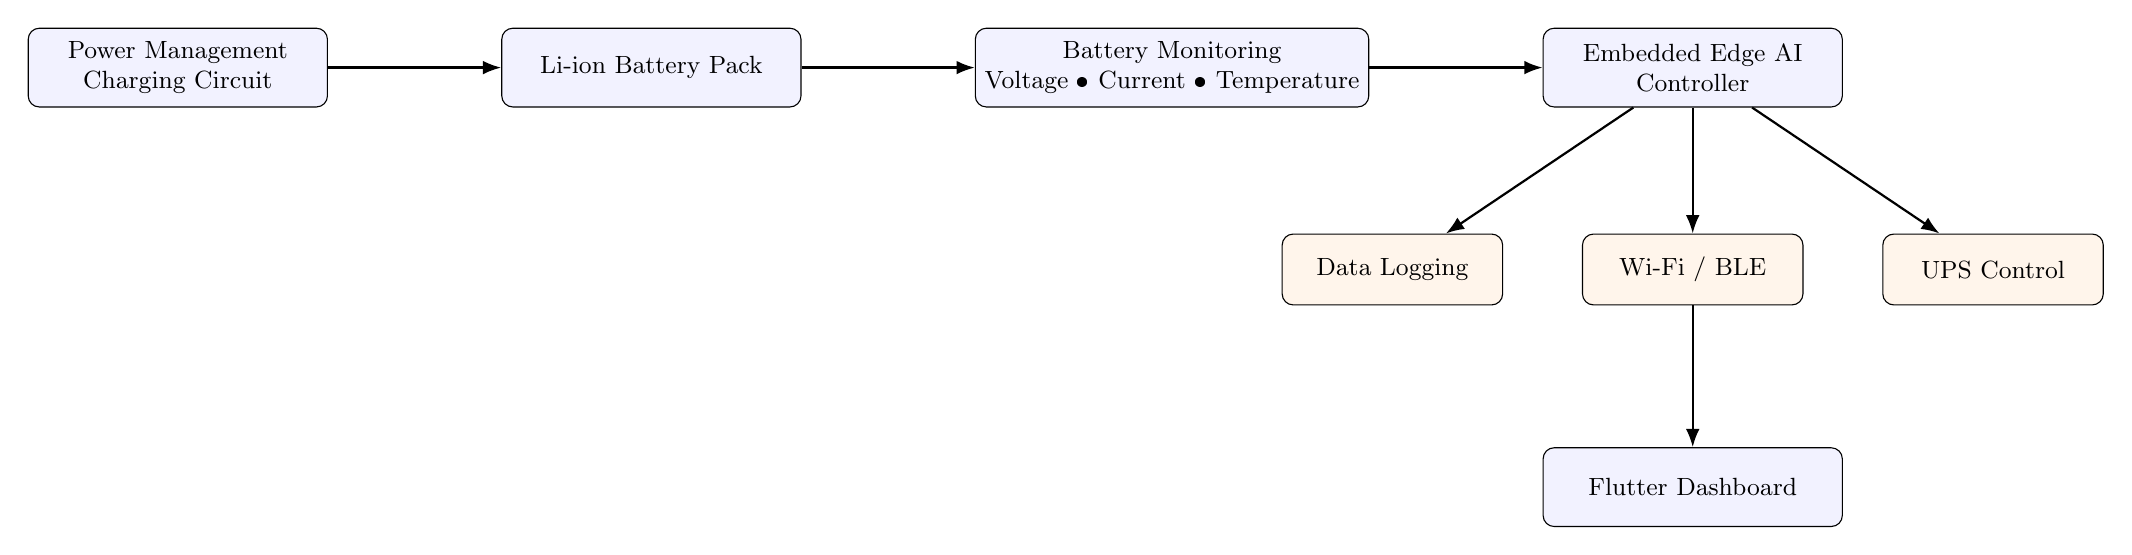
\begin{tikzpicture}[
>=Latex,
node distance=2.0cm,
block/.style={
draw,
rounded corners,
minimum width=3.8cm,
minimum height=1cm,
align=center,
font=\small,
fill=blue!5
},
smallblock/.style={
draw,
rounded corners,
minimum width=2.8cm,
minimum height=0.9cm,
align=center,
font=\small,
fill=orange!8
},
arrow/.style={
-thick,
Latex
}
]

%%%%%%%%%%%%%%%%%%%%%%%%%%%%%%%%%%%%%%%%%%%%%
% Main Blocks
%%%%%%%%%%%%%%%%%%%%%%%%%%%%%%%%%%%%%%%%%%%%%

\node[block] (power)
{Power Management\\
Charging Circuit};

\node[block, right=2.2cm of power] (battery)
{Li-ion Battery Pack};

\node[block, right=2.2cm of battery] (monitor)
{Battery Monitoring\\
Voltage • Current • Temperature};

\node[block, right=2.2cm of monitor] (edge)
{Embedded Edge AI\\
Controller};

%%%%%%%%%%%%%%%%%%%%%%%%%%%%%%%%%%%%%%%%%%%%%
% Outputs
%%%%%%%%%%%%%%%%%%%%%%%%%%%%%%%%%%%%%%%%%%%%%

\node[smallblock, below left=1.6cm and 0.5cm of edge] (log)
{Data Logging};

\node[smallblock, below=1.6cm of edge] (mobile)
{Wi-Fi / BLE};

\node[smallblock, below right=1.6cm and 0.5cm of edge] (ups)
{UPS Control};

\node[block, below=1.8cm of mobile]
(app){Flutter Dashboard};

%%%%%%%%%%%%%%%%%%%%%%%%%%%%%%%%%%%%%%%%%%%%%
% Connections
%%%%%%%%%%%%%%%%%%%%%%%%%%%%%%%%%%%%%%%%%%%%%

\draw[->,thick] (power)--(battery);

\draw[->,thick] (battery)--(monitor);

\draw[->,thick] (monitor)--(edge);

\draw[->,thick] (edge)--(log);

\draw[->,thick] (edge)--(mobile);

\draw[->,thick] (edge)--(ups);

\draw[->,thick] (mobile)--(app);

\end{tikzpicture}%
}

\vspace{0.3cm}
\begin{figure}[ht]
  \centering
  \caption{\textit{Figure: Block diagram of the Edge AI Smart Battery Management System.}}
  \label{fig:topic1_block}
\end{figure}
\end{frame}

\begin{frame}{Topic 1: Expected Outcomes}
\begin{itemize}
  \item A standalone, fully operational \textbf{Edge AI Smart Battery Management System}.
  \vspace{0.25cm}
  \item High-precision \textbf{real-time monitoring} of critical cell voltage, load current, and pack temperature parameters.
  \vspace{0.25cm}
  \item Accurate estimation algorithms for \textbf{State of Charge (SOC)} and \textbf{State of Health (SOH)}, alongside proactive \textbf{RUL forecasting}.
  \vspace{0.25cm}
  \item Automated \textbf{on-device fault detection} linked to immediate, glitch-free UPS backup mode transitions.
  \vspace{0.25cm}
  \item An intuitive, cross-platform \textbf{Flutter monitoring dashboard} displaying comprehensive analytical graphs and alerts.
\end{itemize}
\end{frame}

\begin{frame}{Topic 1: Applications}
\begin{itemize}
  \item \textbf{Electric Vehicles (EVs):} Ensuring enhanced battery pack safety and precise driving range estimation.
  \vspace{0.25cm}
  \item \textbf{Renewable Energy Storage:} Managing residential and municipal solar/wind battery banks efficiently.
  \vspace{0.25cm}
  \item \textbf{Smart UPS Systems:} Uninterruptible power supplies with real-time health diagnostics and automated self-tests.
  \vspace{0.25cm}
  \item \textbf{Industrial Robotics \& AGVs:} Maximizing runtime and lifespan of autonomous factory fleet batteries.
  \vspace{0.25cm}
  \item \textbf{Mission-Critical Backup:} Telecommunication base stations and medical ICU power backup units.
\end{itemize}
\end{frame}

%================ TOPIC 2 ================
\begin{frame}
  \begin{block}{\centering \huge Topic 2}
    \vspace{0.3cm}
    \centering \Large \textbf{Embedded Electronics Diagnostic Instrument}
    \vspace{0.3cm}
  \end{block}
\end{frame}

\begin{frame}{Topic 2: Introduction}
\begin{itemize}
  \item \textbf{Multi-Functional Unit:} A compact, portable diagnostic instrument merging a digital oscilloscope, logic analyzer, and multi-protocol decoder into one standalone device.
  \vspace{0.25cm}
  \item \textbf{Protocol Decoding Support:} Designed to analyze, inspect, and translate standard embedded communication protocols including UART, SPI, I2C, and automotive CAN buses.
  \vspace{0.25cm}
  \item \textbf{Core Capabilities:} Facilitates real-time waveform visualization, precise automated signal parameter measurements, and sustained data logging.
  \vspace{0.25cm}
  \item \textbf{Wireless Connectivity:} Transmits live high-speed diagnostic streams wirelessly to a companion smartphone/PC Flutter application for advanced analysis.
\end{itemize}
\end{frame}

\begin{frame}{Topic 2: Problem Statement}
\begin{itemize}
  \item \textbf{High Cost \& Bulkiness:} Commercial oscilloscopes and logic analyzers are highly expensive, heavy, and practically restricted to indoor lab work-benches.
  \vspace{0.35cm}
  \item \textbf{Accessibility Gap:} Students, field technicians, and R\&D engineers often struggle without portable, reliable debugging gear during field deployment or remote fieldwork.
  \vspace{0.35cm}
  \item \textbf{Proposed Need:} An affordable, compact, handheld diagnostic instrument capable of capturing analog test waveforms and interpreting digital bus traffic simultaneously on a single embedded hardware platform.
\end{itemize}
\end{frame}

\begin{frame}{Topic 2: Proposed Methodology}
\begin{itemize}
  \item \textbf{Signal Acquisition:} High-speed analog front-end circuitry captures and buffers analog and digital signals from the Device Under Test (DUT).
  \vspace{0.25cm}
  \item \textbf{Embedded Processing:} An onboard microcontroller performs real-time sampling, hardware digital filtering, and structural protocol decoding.
  \vspace{0.25cm}
  \item \textbf{Dual-Stage Visualization:} Basic signal indicators can be checked locally on the device, while raw stream data is broadcast over Wi-Fi / Bluetooth Low Energy (BLE).
  \vspace{0.25cm}
  \item \textbf{Interactive Dashboard:} A custom Flutter software client receives the data stream, providing waveform zoom, trigger thresholds, hex protocol tables, and export capabilities.
\end{itemize}
\end{frame}

\begin{frame}{Topic 2: Block Diagram}
\centering
\resizebox{0.75\linewidth}{!}{%
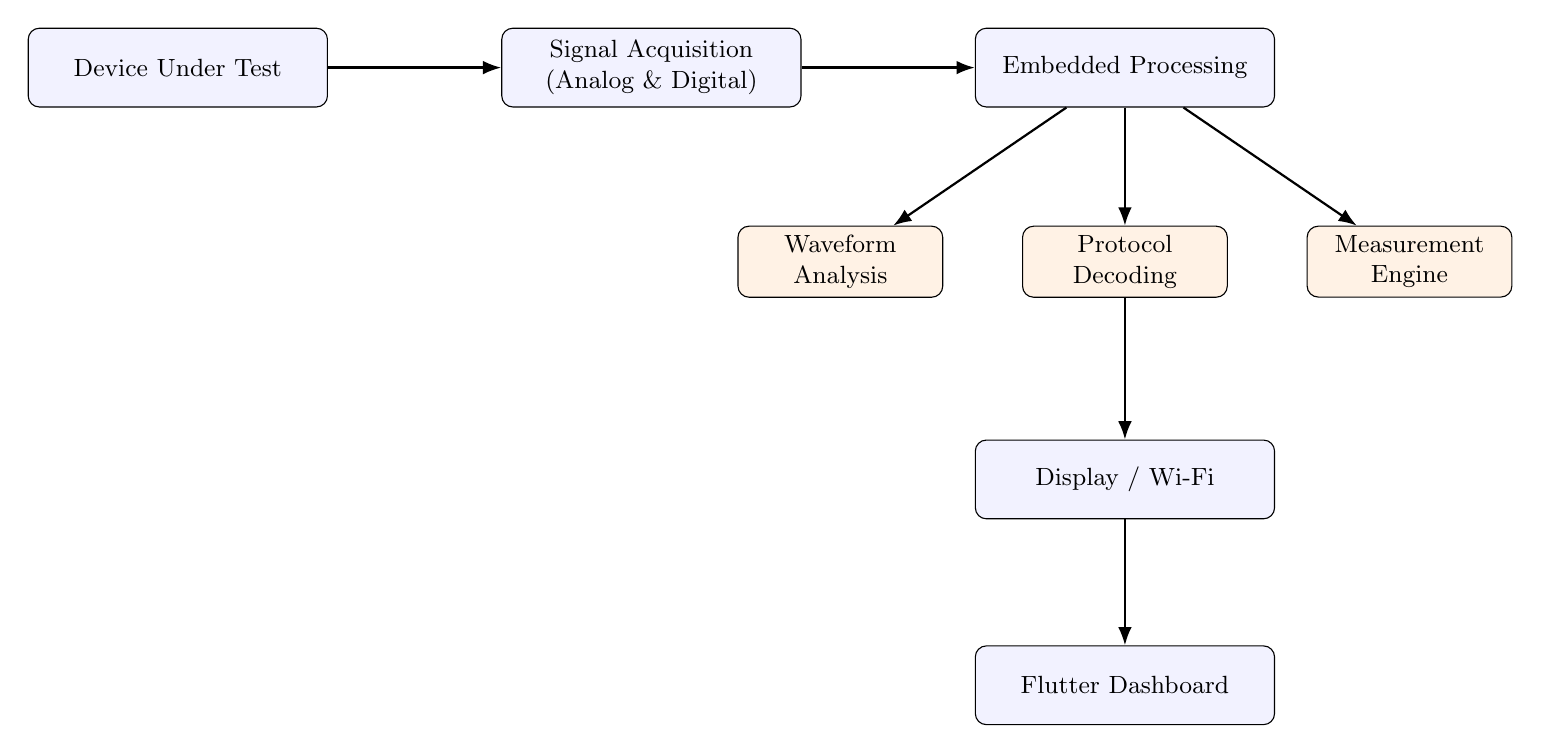
\begin{tikzpicture}[
>=Latex,
node distance=2.3cm,
block/.style={
draw,
rounded corners,
minimum width=3.8cm,
minimum height=1cm,
align=center,
font=\small,
fill=blue!5
},
smallblock/.style={
draw,
rounded corners,
minimum width=2.6cm,
minimum height=0.9cm,
align=center,
font=\small,
fill=orange!10
}
]

%%%%%%%%%%%%%%%%%%%%%%%%%%%%%%%%%%%%
% Main Blocks
%%%%%%%%%%%%%%%%%%%%%%%%%%%%%%%%%%%%

\node[block] (dut)
{Device Under Test};

\node[block,right=2.2cm of dut] (acq)
{Signal Acquisition\\
(Analog \& Digital)};

\node[block,right=2.2cm of acq] (proc)
{Embedded Processing};

%%%%%%%%%%%%%%%%%%%%%%%%%%%%%%%%%%%%
% Processing Outputs
%%%%%%%%%%%%%%%%%%%%%%%%%%%%%%%%%%%%

\node[smallblock,below left=1.5cm and 0.4cm of proc] (wave)
{Waveform\\Analysis};

\node[smallblock,below=1.5cm of proc] (proto)
{Protocol\\Decoding};

\node[smallblock,below right=1.5cm and 0.4cm of proc] (measure)
{Measurement\\Engine};

%%%%%%%%%%%%%%%%%%%%%%%%%%%%%%%%%%%%
% Output
%%%%%%%%%%%%%%%%%%%%%%%%%%%%%%%%%%%%

\node[block,below=1.8cm of proto] (display)
{Display / Wi-Fi};

\node[block,below=1.6cm of display]
(app){Flutter Dashboard};

%%%%%%%%%%%%%%%%%%%%%%%%%%%%%%%%%%%%
% Connections
%%%%%%%%%%%%%%%%%%%%%%%%%%%%%%%%%%%%

\draw[->,thick] (dut)--(acq);

\draw[->,thick] (acq)--(proc);

\draw[->,thick] (proc)--(wave);

\draw[->,thick] (proc)--(proto);

\draw[->,thick] (proc)--(measure);

\draw[->,thick] (proto)--(display);

\draw[->,thick] (display)--(app);

\end{tikzpicture}%
}

\vspace{0.3cm}
\begin{figure}[ht]
  \centering
  \caption{\textit{Figure: Block diagram of the Embedded Electronics Diagnostic Instrument.}}
  \label{fig:topic2_block}
\end{figure}
\end{frame}

\begin{frame}{Topic 2: Expected Outcomes}
\begin{itemize}
  \item A low-cost, pocket-sized \textbf{embedded diagnostic instrument} uniting digital oscilloscope and multi-channel logic analyzer functionalities.
  \vspace{0.3cm}
  \item A dedicated \textbf{real-time protocol decoder} translating UART, SPI, I2C, and CAN messages into readable hexadecimal and text transcripts.
  \vspace{0.3cm}
  \item Reliable \textbf{wireless transmission and data logging} directly to mobile devices or laptops via an aesthetically designed Flutter interface.
  \vspace{0.3cm}
  \item An all-in-one educational and industrial troubleshooting tool ideal for hardware debugging and student lab instruction.
\end{itemize}
\end{frame}

\begin{frame}{Topic 2: Applications}
\begin{itemize}
  \item \textbf{Embedded Firmware Development:} Verifying sensor timing, chip select signals, and SPI/I2C peripheral communication.
  \vspace{0.3cm}
  \item \textbf{PCB Debugging \& Maintenance:} Rapid diagnostic tracing on industrial control boards during field repairs.
  \vspace{0.3cm}
  \item \textbf{Automotive Diagnostics:} Monitoring vehicular CAN bus networks, ECU traffic, and dashboard sensor telemetry.
  \vspace{0.3cm}
  \item \textbf{Academic Laboratories \& Robotics:} Empowering students to run oscilloscope experiments and test robotic circuit hardware anywhere.
\end{itemize}
\end{frame}

%================ TOPIC 3 ================
\begin{frame}
  \begin{block}{\centering \huge Topic 3}
    \vspace{0.3cm}
    \centering \Large \textbf{Adaptive LoRa Mesh Emergency Communication Network}
    \vspace{0.3cm}
  \end{block}
\end{frame}

\begin{frame}{Topic 3: Introduction}
\begin{itemize}
  \item \textbf{Off-Grid Lifeline:} An Adaptive LoRa Mesh Network engineered to guarantee long-range emergency communication when conventional cellular towers and internet infrastructure collapse.
  \vspace{0.25cm}
  \item \textbf{Autonomous Self-Organization:} Distributed handheld and stationary LoRa radio nodes autonomously discover peers and organize into a decentralised, self-healing wireless mesh topology.
  \vspace{0.25cm}
  \item \textbf{Dynamic Packet Routing:} Messages and critical distress alerts dynamically hop across intermediary relay nodes to span large geographical disaster zones.
  \vspace{0.25cm}
  \item \textbf{Integrated Features:} Embeds live GPS tracking, smartphone connectivity via Bluetooth, and dynamic priority routing for search-and-rescue teams.
\end{itemize}
\end{frame}

\begin{frame}{Topic 3: Problem Statement}
\begin{itemize}
  \item \textbf{Infrastructure Vulnerability:} Conventional emergency response depends heavily on terrestrial cellular networks, fiber optic trunks, and grid power—all of which regularly fail during severe floods, earthquakes, and cyclones.
  \vspace{0.35cm}
  \item \textbf{Isolation in Disaster Zones:} Affected communities and deployed first responders experience total communication blackouts, delaying critical search and medical rescues.
  \vspace{0.35cm}
  \item \textbf{Proposed Need:} A fully portable, independent, self-healing, and energy-efficient long-range communication architecture capable of maintaining robust messaging without conventional telecom grids.
\end{itemize}
\end{frame}

\begin{frame}{Topic 3: Proposed Methodology}
\begin{itemize}
  \item \textbf{Mesh Topology Discovery:} Each LoRa transceiver node continuously emits heartbeat broadcasts, exchanging routing metrics to establish a reliable, self-organizing mesh network.
  \vspace{0.25cm}
  \item \textbf{Intelligent Multi-Hop Routing:} Distress broadcasts and chat texts are dynamically routed across optimal hop pathways toward active rescue command stations.
  \vspace{0.25cm}
  \item \textbf{Smartphone Bluetooth Gateway:} Civilians and responders pair smartphones to local LoRa nodes via Bluetooth, composing text alerts through a native mobile application.
  \vspace{0.25cm}
  \item \textbf{Central Command Telemetry:} A designated central command receiver consolidates incoming packets, displaying interactive GPS maps, SOS distress coordinates, and sensor alerts on a Flutter dashboard.
\end{itemize}
\end{frame}

\begin{frame}{Topic 3: Block Diagram}
\centering
\resizebox{0.8\linewidth}{!}{%
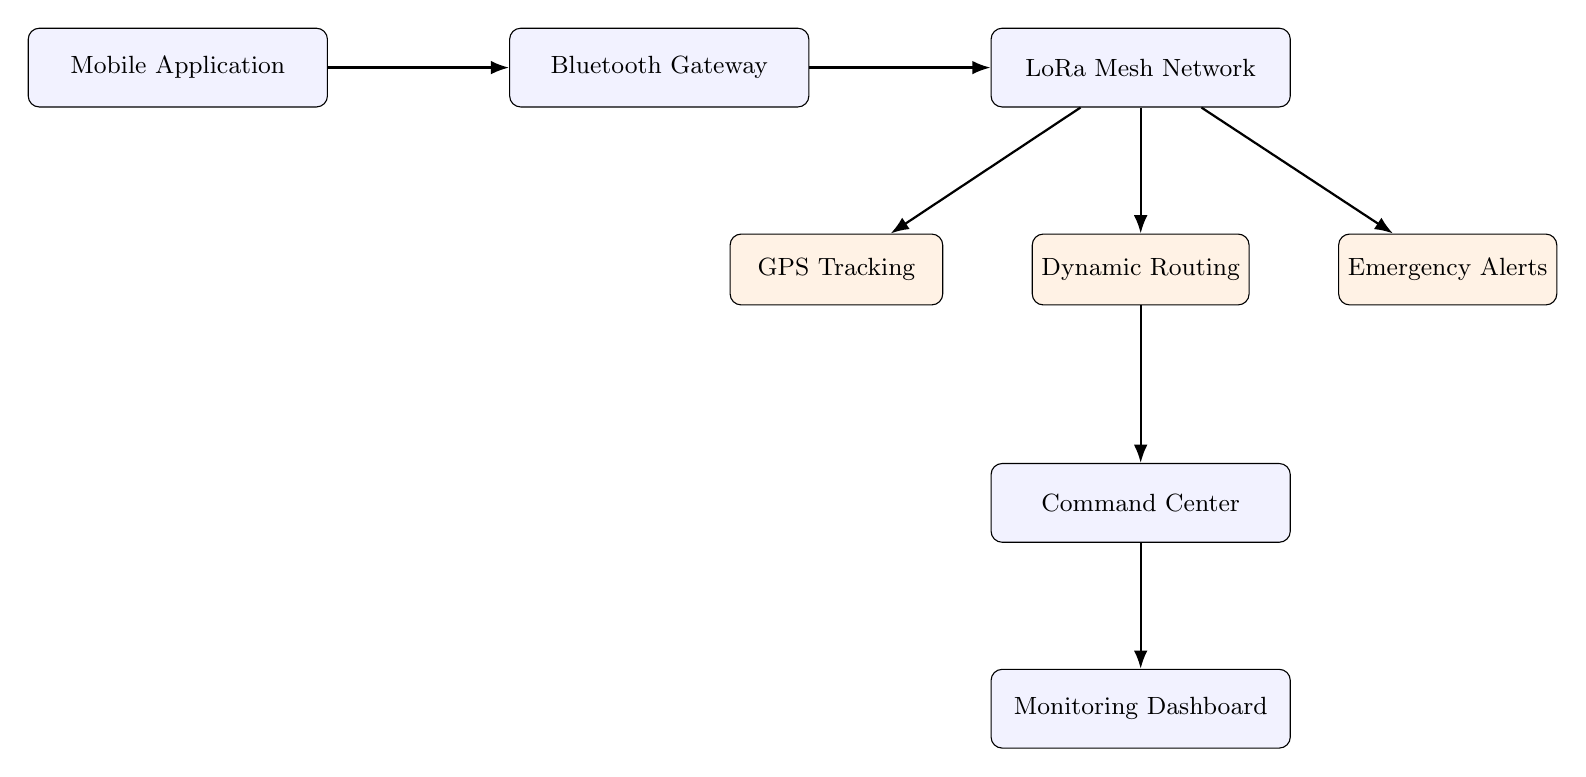
\begin{tikzpicture}[
>=Latex,
node distance=2.3cm,
block/.style={
draw,
rounded corners,
minimum width=3.8cm,
minimum height=1cm,
align=center,
font=\small,
fill=blue!5
},
smallblock/.style={
draw,
rounded corners,
minimum width=2.7cm,
minimum height=0.9cm,
align=center,
font=\small,
fill=orange!10
}
]

%%%%%%%%%%%%%%%%%%%%%%%%%%%%%%%%%%%%%%%%%%%%%
% Main Blocks
%%%%%%%%%%%%%%%%%%%%%%%%%%%%%%%%%%%%%%%%%%%%%

\node[block] (mobile)
{Mobile Application};

\node[block,right=2.3cm of mobile] (gateway)
{Bluetooth Gateway};

\node[block,right=2.3cm of gateway] (mesh)
{LoRa Mesh Network};

%%%%%%%%%%%%%%%%%%%%%%%%%%%%%%%%%%%%%%%%%%%%%
% Mesh Functions
%%%%%%%%%%%%%%%%%%%%%%%%%%%%%%%%%%%%%%%%%%%%%

\node[smallblock,below left=1.6cm and 0.6cm of mesh] (gps)
{GPS Tracking};

\node[smallblock,below=1.6cm of mesh] (routing)
{Dynamic Routing};

\node[smallblock,below right=1.6cm and 0.6cm of mesh] (alerts)
{Emergency Alerts};

%%%%%%%%%%%%%%%%%%%%%%%%%%%%%%%%%%%%%%%%%%%%%
% Monitoring
%%%%%%%%%%%%%%%%%%%%%%%%%%%%%%%%%%%%%%%%%%%%%

\node[block,below=2cm of routing] (center)
{Command Center};

\node[block,below=1.6cm of center] (dashboard)
{Monitoring Dashboard};

%%%%%%%%%%%%%%%%%%%%%%%%%%%%%%%%%%%%%%%%%%%%%
% Connections
%%%%%%%%%%%%%%%%%%%%%%%%%%%%%%%%%%%%%%%%%%%%%

\draw[->,thick] (mobile)--(gateway);

\draw[->,thick] (gateway)--(mesh);

\draw[->,thick] (mesh)--(gps);

\draw[->,thick] (mesh)--(routing);

\draw[->,thick] (mesh)--(alerts);

\draw[->,thick] (routing)--(center);

\draw[->,thick] (center)--(dashboard);

\end{tikzpicture}%
}

\vspace{0.3cm}
\begin{figure}[ht]
  \centering
  \caption{\textit{Figure: Block diagram of the Adaptive LoRa Mesh Emergency Communication Network.}}
  \label{fig:topic3_block}
\end{figure}
\end{frame}

\begin{frame}{Topic 3: Expected Outcomes}
\begin{itemize}
  \item A decentralised, functional \textbf{LoRa mesh communication network} governed by intelligent self-healing routing algorithms.
  \vspace{0.3cm}
  \item Reliable \textbf{long-range, off-grid text messaging} and emergency broadcast capability without SIM cards or cellular connectivity.
  \vspace{0.3cm}
  \item Real-time \textbf{GPS location tracking} and hazard sensor data aggregation across active mobile nodes in the disaster zone.
  \vspace{0.3cm}
  \item An interactive \textbf{Flutter mobile client and command center GIS dashboard} for streamlined tactical disaster response.
\end{itemize}
\end{frame}

\begin{frame}{Topic 3: Applications}
\begin{itemize}
  \item \textbf{Disaster Management \& Rescue:} Lifeline communication during severe floods, earthquakes, landslides, and extreme typhoons.
  \vspace{0.3cm}
  \item \textbf{Remote \& Forest Surveillance:} Coordinating wild-land firefighters and tracking personnel across expansive forests without cellular coverage.
  \vspace{0.3cm}
  \item \textbf{Tactical \& Military Operations:} Establishing rapid, secure, ad-hoc wireless communication grids for reconnaissance deployments.
  \vspace{0.3cm}
  \item \textbf{Smart Agriculture \& Deep IoT:} Connecting remote agro-meteorological stations across expansive rural farmlands.
\end{itemize}
\end{frame}

%---------------- Conclusion / Thank You ----------------
\begin{frame}{}
    \begin{center}
      \begin{huge}
          \textbf{THANK YOU}
      \end{huge}
      \vspace{0.5cm}
      \par\Large Questions \& Discussion
    \end{center}
\end{frame}

\end{document}
